\section{Trust Model}
\label{sec:trust-model}

In the following chapter we will often refer to entities and components as
``trusted'' and ``untrusted''. This trust relation is defined from the
perspective of the data owner as this role is in possession of the sensitive
data.

\subsection{Roles}

\begin{description}
  \item[Infrastructure and Service Provider]
    The infrastructure provider is responsible for the availability of the
    infrastructure used to provide compute, networking, and storage resources.
    As such the infrastructure controls and has access to the physical hardware
    and firmware.

    On the other hand the service provider is responsible for managing services
    that utilize the infrastructure provided by the infrastructure provider in
    order to ease the development and deployment of workloads. As such the
    service provider is not only responsible for deploying the applications, but
    also to provide services that allow the retrieval of attestation evidence
    and initialize TEE environments.

  \item[Application Owner]
    The application owner designs and implements application workloads that will
    be deployed and orchestrated by the service provider. This role needs to
    prove to the customer aspects of compliance to the defined requirements. It
    also defines computing resource requirements for the application workloads
    in order to run and maintain compliance.

  \item[Data Owner]
    As the owner of the confidential data, this role is concerned with the
    visibility and integrity of their data and the compliance of the application
    with the requested requirements.

  \item[Verifier]
    In order to remove the service provider from the application's trust model,
    an external party has to verify the service provider's confidentiality
    claims. The verifier provides an attestation service that appraises evidence
    and returns attestation results.
\end{description}

While the application owner and verifier have to be trusted by the data owner,
the goal is to be able to outsource the management infrastructure and
orchestration of applications, while not having to trust the infrastructure or
service provider. This implies that the entities that take on the role of
infrastructure or service provider should not also be assigned the role of
application owner or verifier.

Roles that have the same trust status can be aggregated into the same entity.
For example the infrastructure provider can at the same time be the service
provider and the roles application owner, data owner, and verifier can be
incorporated into the same entity.

\section{Architecture}
\label{sec:proposal:architecture}

\subsection{Overview}

For convenience, from now on we will refer to confidential data as ``secrets''.
Figure \ref{fig:proposal:architecture-overview} shows an overview over the
components used in this architecture proposal, aiding the reader with
understanding the relation between the components introduced in the next
section.

\begin{figure}[ht]
  \centering
  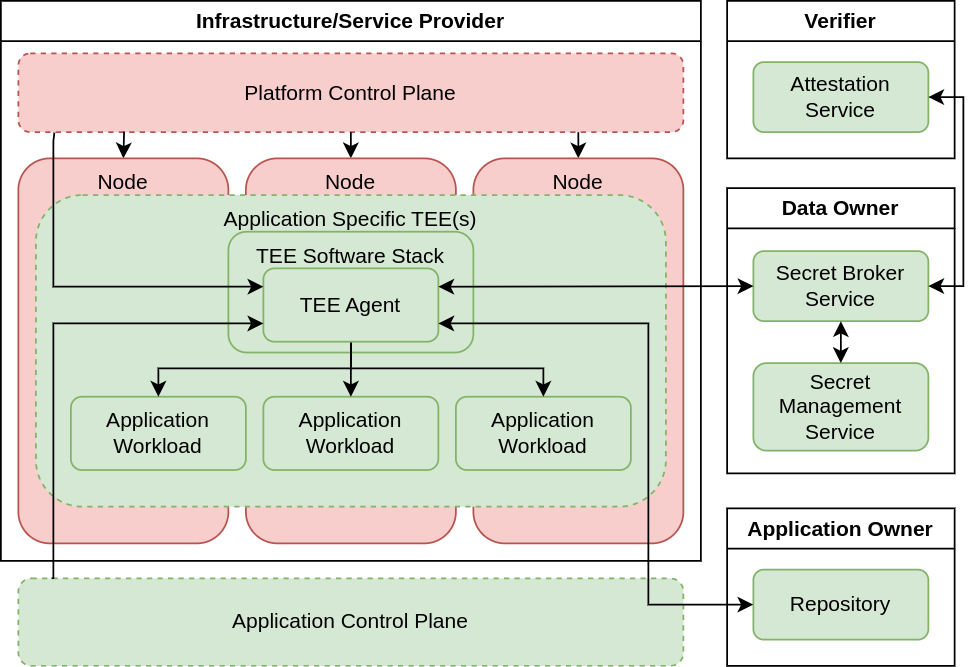
\includegraphics[width=\linewidth]{resources/architecture-overview.png}
  \caption[A simplified overview over the Confidential Containers architecture]{
    An overview over components used in this architecture proposal. Defines
    which components are managed by which role and whether it is trusted.
    Entities and Components marked in red are untrusted, while those marked in
    green are trusted.}
  \label{fig:proposal:architecture-overview}
\end{figure}

\subsection{Components}

\subsubsection{Control Planes}

In a dynamically provisioned platform managing the infrastructure and
orchestrating applications is the responsibility of the control plane. We are
grossly simplifying the control plane here by considering it as a single
component. In traditional platforms the control plane is a high-privileged
component in order to perform management and orchestration tasks.

We want to apply the least privileges principle to the control plane and only
allow privileges necessary for basic management and orchestration. This includes
managing the lifecycle of applications on a node, migration of applications
between nodes, and monitor computing resource usage. But privileges that have
the potential to compromise the integrity of application code and data should
only be assigned to trusted entities and components. This implies that entities
and components controlled by the service provider should not have these
privileges.

To achieve this the traditional control plane has to be split into a platform
and an application control plane. As stated above the platform control plane
manages and orchestrates the platform with only the set of permissions that is
needed to achieve this. On the other hand the application control plane is
responsible for everything that directly interacts with the application. To make
the split of the control plane effective the service provider can not control or
have access to the application control plane. This implies that an external
entity like the application or data owner has to manage this control plane
instance.

\subsubsection{TEE Agent}

TEEs are designed to shield everything within the environment from the outside.
Because the control plane is not part of a specific application TEE, the control
plane is not able to interact with applications inside a TEE. To allow and
control interactions with between the control plane and applications a new
component is needed. The TEE agent itself is executed inside a TEE -- not
necessarily the same TEE as the application -- and is responsible for managing
the application specific workloads. It controls the access into the application
TEE in order to perform management and orchestration actions and is responsible
for enforcing the split control planes' permissions.

In a more traditional platform each node inside a platform cluster runs an agent
which manages the applications running on the particular node. But because the
node is under the control of the infrastructure or service provider the node and
everything running on it can not be trusted. This is why an application specific
agent is needed.

The TEE agent is the trusted component that is responsible for the whole
attestation workflow. It is responsible for pulling application code, verifying
the integrity of the code, executing application code inside a TEE, and
injecting secrets into the application TEE. As such the enclave agent itself has
to be verified before sending secrets to it. In section
\ref{sec:proposal:attestation-workflow} we will go more into detail how this
verification of the TEE agent and application code is performed.

\subsubsection{Repository}

In order to mitigate supply chain attacks the application owner has to store
application code in a trusted signed repository or sign the application code
itself. This signature then has to be validated by the TEE agent before
executing the code on confidential data.

\subsubsection{Secret Management Service}

The secret management service is a component that stores confidential data and
controls the access this data. The management of this service has to be done by
the data owner or delegated to a trusted entity.

\subsubsection{Secret Broker Service}

The secrets broker service receives secrets requests from the TEE agent with
evidence about its own integrity. This evidence is then forwarded to the
attestation service which returns attestation results on which the secrets
broker service then decides whether to trust the TEE agent. If the TEE agent is
trusted the secret broker service then relays the secrets from the secret
management service to the TEE agent.

\subsubsection{Attestation Service}

In the RATS architecture the attestation service takes on the role of the
verifier. It appraises evidence from the TEE agent and returns attestation
results to the secret broker service. See section \ref{sec:rats} for more
information about how the appraisal of evidence is performed.

\section{Attestation Workflow}
\label{sec:proposal:attestation-workflow}

Following is the workflow when the deployment of an application is requested:

\begin{enumerate}
  \item The platform control plane spawns a new TEE on an arbitrary node.
  \item After initialization of the TEE the whole TEE software stack is
        measured.
  \item The measurements are then sent as evidence to the secret broker service.
  \item The secret broker service lets the attestation appraise the evidence and
        then decides whether to trust the TEE agent.
  \item If the agent is trusted the secret broker service queries needed secrets
        from the secret management service and sends them to the TEE agent.
        These secrets have to include repository or application code signatures.
  \item After receiving the secrets the TEE downloads application code from the
        repository and verifies it with the signatures it received.
  \item The TEE agent then starts the application workloads in a TEE. This could
        be the same TEE where the agent is running or a new workload specific
        TEE.
\end{enumerate}
